%!TEX program = xelatex
\documentclass{CQUPTThesis}
\title{测试文本}
\author{朱权威}

\usepackage{graphicx} 
\usepackage{amsmath}
\usepackage{algorithm}  
\usepackage{algorithmic}


\begin{document} 
% \maketitle
% \hline
%  & 分类号 &  & 密级 &  \\ \hline
%  & UDC &  & 学位论文编号 &  \\ \hline
% \cntitle{重庆邮电大学硕士学位论文写作模板}
% \entitle{Thesis Templatefor Master’s \\Degree of Chongqing University University of Posts and Telecommunications}
% \stuno{S160231097}
% \name{朱权威}
% \degree{工程硕士}
% \subject{计算机技术}
% \tutor{米建勋}
% \tutortitle{副教授}
% \finishdate{2017年11月29日}
% \makecover
% \clearify
\cAbstract{
学位论文是研究生从事科研工作的成果的主要表现,它集中表明了作者在研究
工作中获得的新发明、新理论或新见解,是研究生申请学位的重要依据,也是科研
领域中的重要文献资料和社会的宝贵财富。为了提高研究生学位论文的质量,做到
学位论文在内容和格式上的规范化与统一化,特制作本模板。

“摘要”二字为黑体三号字居中,是一级标题。摘要与内容之间不空行,摘要内容与关键词间空一行。“关键词”三个字采用宋体小四号字加粗。摘要内容和关键词采用中文宋体、英文Times New Roman,小四号字,1.5倍行距。关键词是为了文献标引工作从论文中选取出来用以表示全文主题内容信息的单词或术语。

关键词是为了文献标引工作从论文中选取出来用以表示全文主题内容信息的单词或术语。自定义3-5个关键词,按外延由大到小排列,建议采用EI标准检索词,关键词间用逗号分开。如有可能,应尽量用《汉语主题词表》等词表提供的规范词。
\ckeyword{学位论文,论文格式,规范化,模板}
}


\Abstract{Thesis is postgraduate’s main academic performance to display her/his works of
scientific research, which shows the author’s new invention, new theory or new opinion
in her/his research. It is the crucial document for the graduate students to apply for degree,
and it is also the important scientific research literature and the valuable wealth of society.
In order to improve the quality of postgraduate’s thesis, this template is formulated to
standardize and unify the thesis’s content and format
\keyword{thesis, format, standardization, template}}

%目录
\maketoc

\renewcommand{\chaptermark}[1]{\markboth{#1}{}}
%图录,表录,不需要可以注释掉

 \listoffigures
 \addcontentsline{toc}{chapter}{图录}
 \listoftables
 \addcontentsline{toc}{chapter}{表录}
\makenote
 \begin{note}
\item[PCA] pca
\item[Pitemize] addddddd
\end{note}
 \mainmatter



\chapter{标题}
hello 中文 texlatex论文页边距按以下标准设置论文页边距按以下标准设置论文页边距按以下标准设置
学位论文页边距按以下标准设置:上边距(天showframe头)3 厘米,下边距(地脚)2.5
厘米,左右边距 2.5 厘米,装订线靠
\section{测试}
左 1 厘米,页眉顶端距离 1.6 厘米,页脚底端
距离 1.5 厘米。无网格。

\section{测试}
\subsection{字体}
左 1 厘米,页眉顶端距离 1.6 厘米,页脚底端
距离 1.5 厘米。无网格。
\subsection{换行English}
左 1 厘米,页眉顶端距离 1.6 厘米,页脚底端English
距离 1.5 厘米。无网格。左 1 厘米,页眉顶端距离 1.6 厘米,页脚底端
距离 1.5 厘米。无网格。

\subsubsection{张English}
距离 1.5 厘米。无网格。左 1 厘米,页眉顶端距离 1.6 厘米,页脚底端
距离 1.5 厘米。无网格。
\subsubsection{里}
距离 1.5 厘米。无网格。左 1 厘米,页眉顶端距离 1.6 厘米,页脚底端
距离 1.5 厘米。无网格。
123
\section{换行}
左 1 厘米,页眉顶端距离 1.6 厘米,页脚底端
\subsubsection{章}
题,中文黑体、英文
距离 1.5 厘米。无网格。
\chapter{图表示例}
论文正文的中文字体用宋体;英文字体

则要求为 Times New Roman。正文中
的文字部分要求两端对齐。
4.4.3 字号

1. 目录题目(目录、图录、表录、注释)——是一级标题,中文黑体、英文
Times New Roman, 3 号字居中,段前 17 磅,段后 16.5 磅,1.5 倍行距;
2. 章标题(第 x 章)——是一级标题,中文黑体、英文 Times New Roman, 3
号字居中,段前 17 磅,段后 16.5 磅,1.5 倍行距;
3. 节标题(x.x)——是二级标题,中文黑体、英文 Times New Roman 小 3 号字
顶格居左,段前 13 磅,段后 13 磅,1.5 倍行距,节名和文字间空 1 个字符,不空
行;
\begin{table}[h]
\centering
\caption{测试表格}
\begin{tabular}{|c|c|c|}
\hline
 &中文&English\\\hline
 &中文&English \\\hline
\end{tabular}
\label{table}
\end{table}

4. 条标题(x.x.x)——是三级标题,中文黑体、英文 Times New Roman4 号字顶
格居左,段前 13 磅,段后 13 磅,1.5 倍行距,条名和文字间空 1 个字符,不空行;
5. 正文——中文宋体、英文 Times New Roman 小 4 号,首行缩进 2 字符,1.5
倍行距;这里是表格引用表.\ref{table}

6. 正文后的题目(参考文献、致谢、攻读 xx 期间发表的论文)——是一级标
题,中文黑体、英文 Times New Roman, 3 号字居中,段前 17 磅,段后 16.5 磅,
1.5 倍行距。这里是图片引用表.\ref{1}

论文中的非学术型错误主要包含错别字、格式错误、图表错误、参考文献格
式错误、序号列表错误、排版问题等被普遍认为的非学术型的低级错误。论文中
存在大量低级错误,说明论文写作质量差,影响读者对其学术水平的判定,同时
也反映了该论文作者缺乏认真、严谨、负责的科学态度和素养,没有达到合格人
才的培养目的。
为进一步规范硕士学位论文撰写,提高论文写作质量,在论文答辩前对研究
生学位论文进行校院两级查非抽查工作。


参加查非的论文要求如下:
1. 通过检测的学位论文的非学术型错误数量为:小于 20 处;
2. 未通过检测且需要二次检测的论文非学术$alpha=1$
则要求为 Times New Roman。正文中
\begin{figure}[htp]
\centering
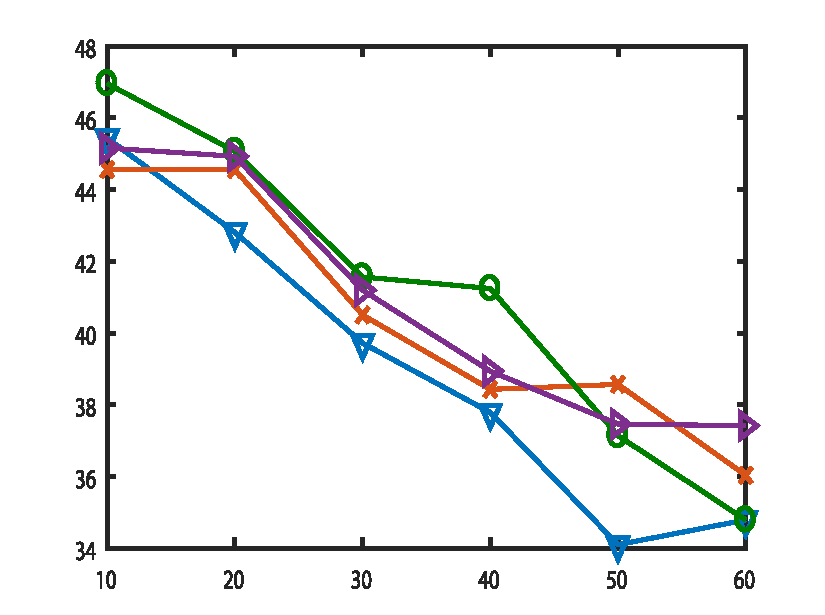
\includegraphics[width=0.8\textwidth]{figures/figure.pdf} 
\caption{测试图片}
\label{1}
\end{figure}
论文中的非学术型错误主要包含错别字、格式错误、图表错误、参考文献格
式错误、序号列表错误、排版问题等被普遍认为的非学术型的低级错误。论文中
存在大量低级错误,说明论文写作质量差,影响读者对其学术水平的判定,同时
也反映了该论文作者缺乏认真、严谨、负责的科学态度和素养,没有达到合格人
才的培养目的。
为进一步规范硕士学位论文撰写,提高论文写作质量,在论文答辩前对研究
生学位论文进行校院两级查非抽查工作。


参加查非的论文要求如下:
1. 通过检测的学位论文的非学术型错误数量为:小于 20 处;
2. 未通过检测且需要二次检测的论文非学术$alpha=1$
则要求为 Times New Roman。正文中

重庆邮电大学硕士学位论文 第 4 章 其他格式要求
19
4.5 论文查非要求

\chapter{Equation}
论文中的非学术型错误主要包含错别字、格式错误、图表错误、参考文献格
式错误、序号列表错误、排版问题等被普遍认为的非学术型的低级错误。论文中
存在大量低级错误,说明论文写作质量差,影响读者对其学术水平的判定,同时
也反映了该论文作者缺乏认真、严谨、负责的科学态度和素养,没有达到合格人
才的培养目的。
为进一步规范硕士学位论文撰写,提高论文写作质量,在论文答辩前对研究
生学位论文进行校院两级查非抽查工作。

论文中的非学术型错误主要包含错别字、格式错误、图表错误、参考文献格
式错误、序号列表错误、排版问题等被普遍认为的非学术型的低级错误。论文中
存在大量低级错误,说明论文写作质量差,影响读者对其学术水平的判定,同时
也反映了该论文作者缺乏认真、严谨、负责的科学态度和素养,没有达到合格人
才的培养目的。
为进一步规范硕士学位论文撰写,提高论文写作质量,在论文答辩前对研究
生学位论文进行校院两级查非抽查工作。


参加查非的论文要求如下:
1. 通过检测的学位论文的非学术型错误数量为:小于 20 处;
2. 未通过检测且需要二次检测的论文非学术$alpha=1$
则要求为 Times New Roman。正文中
\begin{align}
\min\quad&\sum_{i=1}^n\|x_i-WW^\mathrm{T}x_i\|_2^2\label{PCA}\\
\mbox{s.t.} \quad& W^\mathrm{T}W=I\notag
\end{align}
的文字部分要求两端对齐。
\begin{equation}
\|x_i-Wy_i\|_2=\sqrt{x_i^\mathrm{T}x_i-x_i^\mathrm{T}WW^\mathrm{T}x_i}=s_i
\end{equation}
4.4.3 字号

1. 目录题目(目录、图录、表录、注释)——是一级标题,中文黑体、英文
Times New Roman, 3 号字居中,段前 17 磅,段后 16.5 磅,1.5 倍行距;
2. 章标题(第 x 章)——是一级标题,中文黑体、英文 Times New Roman, 3
号字居中,段前 17 磅,段后 16.5 磅,1.5 倍行距;
3. 节标题(x.x)——是二级标题,中文黑体、英文 Times New Roman 小 3 号字
顶格居左,段前 13 磅,段后 13 磅,1.5 倍行距,节名和文字间空 1 个字符,不空
行;
4. 条标题(x.x.x)——是三级标题,中文黑体、英文 Times New Roman4 号字顶
格居左,段前 13 磅,段后 13 磅,1.5 倍行距,条名和文字间空 1 个字符,不空行;
5. 正文——中文宋体、英文 Times New Roman 小 4 号,首行缩进 2 字符,1.5
倍行距;


6. 正文后的题目(参考文献、致谢、攻读 xx 期间发表的论文)——是一级标
题,中文黑体、英文 Times New Roman, 3 号字居中,段前 17 磅,段后 16.5 磅,
1.5 倍行距。
重庆邮电大学硕士学位论文 第 4 章 其他格式要求
19
4.5 论文查非要求

论文中的非学术型错误主要包含错别字、格式错误、图表错误、参考文献格
式错误、序号列表错误、排版问题等被普遍认为的非学术型的低级错误。论文中
存在大量低级错误,说明论文写作质量差,影响读者对其学术水平的判定,同时
也反映了该论文作者缺乏认真、严谨、负责的科学态度和素养,没有达到合格人
才的培养目的。
为进一步规范硕士学位论文撰写,提高论文写作质量,在论文答辩前对研究
生学位论文进行校院两级查非抽查工作。

参加查非的论文要求如下:
1. 通过检测的学位论文的非学术型错误数量为:小于 20 处;
\begin{algorithm}
\linespread{1.0}\selectfont
\caption{RSPCA algorithm}
{\bf Input: }Dataset $X=[x_1,x_2,...,x_n]$, index matrix $D=[D_1,D_2,...D_k]$,and something else.
\label{alg1}
\begin{algorithmic}[1]
  \STATE initial $W,y_i$ with a random vector
  \WHILE{not converge}
  \STATE compute mean $\bar x$ according to Eq.
  \STATE centering dataset $\hat X \leftarrow X - \bar x$
  \STATE minimize  to update $W$
  \STATE minimize  with a fixed $W$ to update $y_i$
  \ENDWHILE 
\end{algorithmic}
{\bf Output:} $W,Y=[y_1,y_2,...,y_n]$
\end{algorithm}
则要求为 Times New Roman。正文中
的文字部分要求两端对齐。
4.4.3 字号

1. 目录题目(目录、图录、表录、注释)——是一级标题,中文黑体、英文
Times New Roman, 3 号字居中,段前 17 磅,段后 16.5 磅,1.5 倍行距;
2. 章标题(第 x 章)——是一级标题,中文黑体、英文 Times New Roman, 3
号字居中,段前 17 磅,段后 16.5 磅,1.5 倍行距;
3. 节标题(x.x)——是二级标题,中文黑体、英文 Times New Roman 小 3 号字
顶格居左,段前 13 磅,段后 13 磅,1.5 倍行距,节名和文字间空 1 个字符,不空
行;
4. 条标题(x.x.x)——是三级标题,中文黑体、英文 Times New Roman4 号字顶
格居左,段前 13 磅,段后 13 磅,1.5 倍行距,条名和文字间空 1 个字符,不空行;
5. 正文——中文宋体、英文 Times New Roman 小 4 号,首行缩进 2 字符,1.5
倍行距;


6. 正文后的题目(参考文献、致谢、攻读 xx 期间发表的论文)——是一级标
题,中文黑体、英文 Times New Roman, 3 号字居中,段前 17 磅,段后 16.5 磅,
1.5 倍行距。
重庆邮电大学硕士学位论文 第 4 章 其他格式要求
19
4.5 论文查非要求

论文中的非学术型错误主要包含错别字、格式错误、图表错误、参考文献格
式错误、序号列表错误、排版问题等被普遍认为的非学术型的低级错误。论文中
存在大量低级错误,说明论文写作质量差,影响读者对其学术水平的判定,同时
也反映了该论文作者缺乏认真、严谨、负责的科学态度和素养,没有达到合格人
才的培养目的。
为进一步规范硕士学位论文撰写,提高论文写作质量,在论文答辩前对研究\cite{RN11,RN27,RN59}
生学位论文进行校院两级查非抽查工作\cite{王宏漫2003采用}。
参加查非的论文要求如下:
1. 通过检测的学位论文的非学术型错误数量为:小于 20 处;



\makebib
\bibliographystyle{hithesis}
\bibliography{ref}

\makeappendix

\chapter{测试}
公会
\chapter{测试}
公会



\thanks{
	致谢二字一级标题:黑体 3 号字居中,段前 17 磅,段后 16.5 磅,1.5 倍行距,
致谢二字与致谢内容之间不空行。致谢内容正文样式:宋体小四号,1.5 倍行距。
}


\achieve{
\bfs{参与科研项目:}
\begin{proj}
	\item 项目名称(编号),项目类别,项目起止很多很多很多很多很多很多很多很多很多很多很多很多文字
	\item 项目名称(编号),项目类别,项目起止
\end{proj}
\bfs{发表及完成论文:}
\begin{proj}
	\item 项目名称(编号),项目类别,项目起止
	\item 项目名称(编号),项目类别,项目起止
\end{proj}
\bfs{获奖:}
\begin{proj}
	\item 项目名称(编号),项目类别,项目起止
	\item 项目名称(编号),项目类别,项目起止
\end{proj}
}
\end{document}